\documentclass{article}
\usepackage[T1]{fontenc}
\usepackage[preprint]{corl_2026}
\usepackage{graphicx,booktabs,xurl}
\hypersetup{
  pdftitle={When Can a Robot Record That an Object Is Gone? A Counterfactual Audit of Two-Image Scene Memory},
  pdfsubject={Research preprint on object removal and occlusion in simulated robot scene memory},
  pdfauthor={Adithya Rajendran}
}
% Generated from archived evidence. Run build.py to regenerate these rows.
\newcommand{\PrimaryRows}{%
  Isaac Sim & 67/80 & 76/80 & $+11.3$ ($+6.3$ to $+16.3$) \\
  MuJoCo & 63/80 & 78/80 & $+18.8$ ($+10.0$ to $+27.5$) \\
}
\newcommand{\CoverageRows}{%
  Isaac Sim & Homography & 387 & 387 & 0 & 0 \\
   & Dense geometry & 397 & 397 & 0 & 0 \\
   & Zero-shot Qwen & 391 & 415 & 24 & 0 \\
  MuJoCo & Homography & 389 & 390 & 1 & 0 \\
   & Dense geometry & 400 & 402 & 2 & 0 \\
   & Zero-shot Qwen & 390 & 417 & 27 & 0 \\
}
\newcommand{\ExactRows}{%
  Isaac Sim & 0/320 & 0 & --- & --- & --- \\
  MuJoCo & 88/320 & 16 & 0/88 & 1/88 & 4/88 \\
}
\newcommand{\DeletionRows}{%
  Homography & 378 (59.1\%) & 1 (0.16\%) & 0 \\
  Dense geometry & 399 (62.3\%) & 2 (0.31\%) & 1 \\
  Zero-shot Qwen & 419 (65.5\%) & 51 (7.97\%) & 4 \\
  STILL, registered crop & 462 (72.2\%) & 36 (5.63\%) & 11 \\
  STILL, conservative crop & 213 (33.3\%) & 3 (0.47\%) & 1 \\
  STILL, scene plus crop & 579 (90.5\%) & 160 (25.00\%) & 79 \\
}


\title{When Can a Robot Record That an Object Is Gone?\\
  A Counterfactual Audit of Two-Image Scene Memory}
\author{Adithya Rajendran\\San Jos\'e State University}

\begin{document}
\maketitle

\begin{abstract}
A panel can conceal a remembered object and its empty location equally well.
We audit a robot's decision to record removal using 1,280 two-image queries from 16 layouts shared by Isaac Sim and MuJoCo, rendering each object both retained and removed at the same camera pose.
After a 6\,cm shift and $3^\circ$ yaw with the blocker parked, dense registration increased correct removal decisions over homography from 67/80 to 76/80 in Isaac Sim and from 63/80 to 78/80 in MuJoCo, but two new false deletions on MuJoCo shelves failed the prespecified improvement criterion.
At 88 fully hidden MuJoCo positions with identical inputs across states, homography abstained on every pair and dense geometry declared removal in both states on one pair.
In a retrospective comparison, trained STILL missed 178 of 640 removals and falsely deleted 36 of 640 retained objects, compared with 221 misses and 51 false deletions for zero-shot Qwen3.5-9B.
STILL deleted both states on 11 of those 88 pairs, illustrating how even a physically correct deletion can lack distinguishing evidence.
\end{abstract}
\keywords{robot scene memory, occlusion, visual verification}

\section{Introduction}

A robot remembers a can on a shelf. On its next visit, a panel covers the place where the can sat.
Should the robot erase the memory? A simulator can tell whether someone removed the can or merely placed the panel in front of it.
The robot can receive exactly the same observation in either case (Figure~\ref{fig:shelf}).

\begin{figure}[htbp]
  \centering
  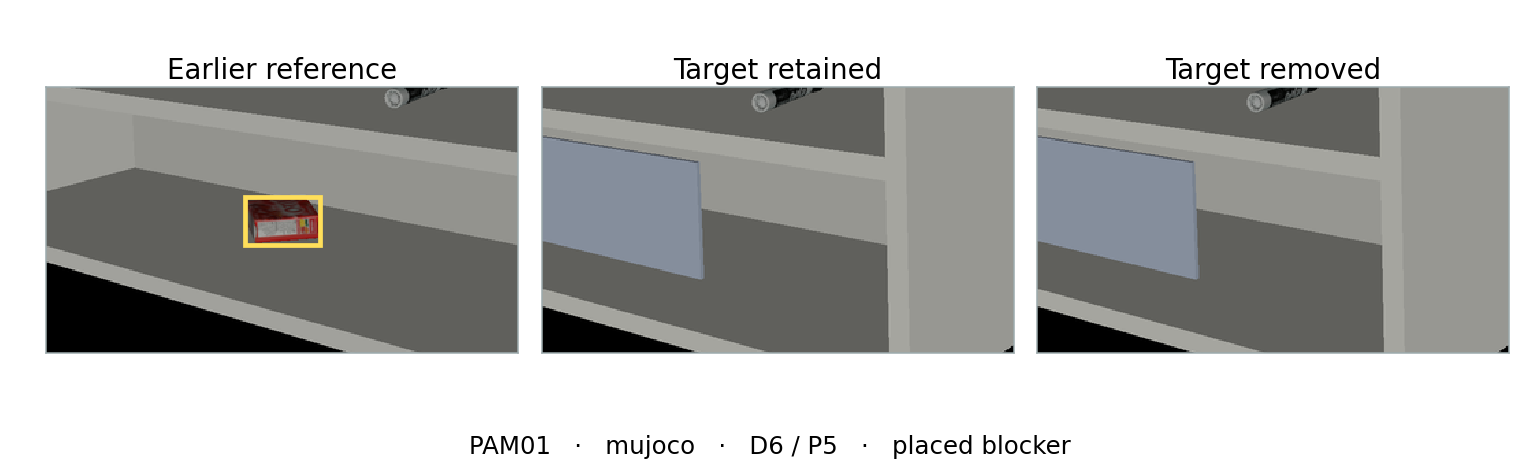
\includegraphics[width=\linewidth]{figures/fresh-matched-pair.png}
  \caption{MuJoCo shelf, layout PAM01, stop P5. The yellow outline marks the earlier gelatin box. It remains behind the panel in the middle image and is absent on the right. The full revisits are pixel-identical. Homography and dense geometry abstained twice. Zero-shot Qwen answered \emph{removed} twice. Trained STILL withheld both deletions because it lacked a registered crop. The original display rule selected this pair.}
  \label{fig:shelf}
\end{figure}

We study one decision in a memory system. A verifier receives an earlier color image, a box around a remembered object, and one later color image.
We measure when it correctly updates a changed record and when it erases a retained object.
A detector that always reports removal succeeds on every clear removal. A verifier that always abstains avoids every false deletion. A useful comparison has to count both outcomes.
Our contribution is an audit that couples the physical intervention to a check of the actual delivered images. It identifies a subset of decisions whose input could equally well have come from the opposite physical state.
Appendix~\ref{app:data} links the exact images, decisions and code for reproducing the comparison.

\section{Related work}

SceneDiff evaluates object changes across visits with different viewpoints~\citep{scenediff}. STILL estimates where a proposed object's former place appears in the other capture and trains a vision-language model to compare the scene and the registered place~\citep{still}. These studies establish the problem of occlusion and the value of registration. We start with a specified object and a supplied reference box. We intervene on that object's presence and ask what a deletion means when the entire input recurs in the opposite state. This endpoint differs from detection average precision, which also reflects proposal generation, ranking and localization.

PBD-AG requires repeated observable misses before removing a stored object~\citep{pbdag}. SafeVantage and VA-TAMP gather further observations for decisions that depend on visibility~\citep{safevantage,vatamp}. BAVO-Bench varies the viewpoint at a fixed scene state~\citep{bavo}. We vary the target state at a fixed viewpoint. This complements selective classification, which evaluates coverage and error together~\citep{reject}. SceneForge shows how an intervention can change shadows and reflections even when the target mesh is hidden~\citep{sceneforge}.

IntPhys uses matched observations to test object permanence, and HuMeGo tests actions that depend on an earlier cue~\citep{intphys,humego}. TRAPSBench, the Counterfactual Memory Audit, SpatialUncertain and VAD-R address answerability, memory or abstention~\citep{trapsbench,cma,spatialuncertain,vad-r}. Here both the earlier cue and the revisit can be identical across interventions. The evaluator can certify ambiguity for those pairs directly. Appendix~\ref{app:related} details the relation to the other tasks.

\section{Counterfactual audit}
\label{sec:design}

\paragraph{What identical inputs establish.}
Let $x=(r,b,q,t)$ contain the decoded reference image, numeric reference box, decoded revisit and fixed task. For each camera and blocker position, we construct $x_P$ with the target retained and $x_R$ with it removed.
If $x_P=x_R$, a deterministic verifier must return the same answer on both. A definite \emph{present} or \emph{removed} answer is physically correct once and wrong once. Neither answer distinguishes the states. Across $c$ such pairs with a definite answer, there are $2c$ unsupported commitments and $c$ physical errors. Abstention makes no update.
This count applies to the balanced intervention design. Unequal pixels alone establish neither visibility nor the ability to decide.

\paragraph{Scenes and interventions.}
The main panel crosses two environments (shelf and tabletop), two targets (gelatin box and large marker), two blocker families (wide panel and white box), and two seeded layouts per combination. The 16 layouts, cameras and assets are shared across the simulators~\citep{ycb,posecnn,isaac,mujoco}.
Each of five camera stops supplies a clear, retained nominal reference. The revisit has the blocker parked or placed and the target retained or removed, at the nominal pose or after a 6\,cm horizontal shift and $3^\circ$ yaw. This gives 640 queries per simulator, half in each target state.
Removal disables target rendering in an otherwise fixed scene. Simulator flags and instance masks establish the physical label. Verifiers receive only RGB and the reference box.
Both decoded images are compared at scoring resolution and separately at native resolution. Appendix~\ref{app:design} gives the seed, rendering and input conventions.

\paragraph{Fixed geometry and zero-shot baselines.}
Homography fits a planar alignment of image edges with the target neighborhood excluded and rejects shifts above 200 input pixels~\citep{ecc}. Dense geometry projects reference locations into the revisit using VGGT estimates of pose and depth and a visibility filter adapted from GeoSCD~\citep{vggt,geoscd}. It abstains when less than 60\% of the reference box has a usable map. Both methods use the same DINOv2 appearance and obstruction checks after registration~\citep{dinov2,yoloworld}.
Our original language-model system sends the full views and two local crops to zero-shot Qwen3.5-9B only after the dense alignment check passes~\citep{qwen,qwen-weights}. Its prompt requests \emph{present}, \emph{removed}, or \emph{unknown}. An archived clear-view screen qualified this system only on clear controls.

\paragraph{Primary comparison and statistical unit.}
Ten separate exploratory layouts informed the choice of comparators and endpoints. The dense adapter failed its development stop rule and was retained at the same settings for this measurement. Local design records predate the new layouts. The protocol and results first appeared together in public Git history.
The primary endpoint is the proportion of all parked-blocker, moved-camera removals answered correctly. Abstentions remain in the denominator. We required a gain in each engine, net gains on at least two tabletop layouts per engine, zero newly wrong definite answers relative to homography anywhere on the panel, and abstention on every certified pair. An engine with no exact pairs leaves the last condition unassessed.
Descriptive 95\% percentile intervals use 10,000 paired resamples of whole layouts within shelf and tabletop strata. Each draw preserves the stops, target states, methods and both engines for a layout.

\paragraph{Trained STILL follow-up.}
After inspecting the original results, we evaluated Xie, Li and Meng's released seed-2 Qwen3.5-9B verifier~\citep{still,still-weights}. Pi3 projects the supplied reference box into the other view from RGB~\citep{pi3}. Our primary STILL rule uses the authors' two red-box crops and the score for \emph{changed}. A missing crop withholds deletion. A below-threshold score keeps the memory without asserting that the object was visible.
We selected the place threshold (0.00071) by maximizing removal F1 on 800 balanced queries from the ten exploratory layouts. We locked it before scoring STILL on the 16 main layouts. No complete image-pair and reference-box combination crossed the split.
Appendix~\ref{app:operating} gives the crop and fusion rules. All results compare complete systems, including their registration, prompts and thresholds.

\section{Results}

\subsection{Clear removals improved, but the geometric change failed its adoption rule}

\begin{table}[htbp]
  \centering
  \caption{Correct removal decisions with the blocker parked after camera motion. Each engine contributed 80 removals from the same 16 layouts. The last column gives the paired difference in percentage points and its 95\% layout interval.}
  \label{tab:primary}
  \begin{tabular}{lrrc}
    \toprule
    Simulator & Homography & Dense geometry & Dense minus homography \\
    \midrule
    \PrimaryRows
    \bottomrule
  \end{tabular}
\end{table}

Dense geometry gained nine correct moved-camera removal decisions and lost none in Isaac Sim. It gained 16 and lost one in MuJoCo (Table~\ref{tab:primary}).
On the tabletop, scores rose from 30/40 to 39/40 in Isaac Sim and from 30/40 to 40/40 in MuJoCo. Six of eight Isaac and seven of eight MuJoCo tabletop layouts improved on balance.
Across all states, the new method introduced two false deletions of retained markers on different MuJoCo shelves. One marker was behind the wide panel. The other had 1,518 native target pixels visible with the blocker parked. Dense geometry avoided a homography error in a third layout. The two new errors failed the prespecified criterion regardless of that avoided error.
Appendix~\ref{app:geometry} gives the per-target and full-panel results.

\subsection{When hidden and removed produced identical evidence}

The target contributed zero native mask pixels at the same 88 of 160 blocker-placed positions in both engines, spanning all 16 layouts. At all 88, MuJoCo produced identical inputs across the retained and removed states. None of the 320 Isaac pairs matched at either resolution. The cause of a pixel difference matters for interpretation. A shadow or renderer variation can change an image even when an object is completely hidden.

Homography abstained on all 88 MuJoCo pairs. Dense geometry abstained on 87. At the remaining shelf position it aligned the blocker to the remembered location, obtained a target similarity of 0.391 and obstruction of 0.167, and declared removal in both states. The original Qwen gate passed four of the 88 pairs. Qwen declared removal on both members of every admitted pair. Figure~\ref{fig:shelf} shows one of them.

\paragraph{Partial exposure.}
In a post hoc analysis, both members of a pair inherit the fraction of the isolated silhouette exposed in the retained twin (Figure~\ref{fig:visibility}). At 50\% to below 90\% exposure, five layouts supplied 28 pairs. Homography identified 19/28 retained targets and 12/28 removals, with one false deletion. Dense geometry identified 1/28 retained targets and 3/28 removals and abstained on the other 52 queries. The clear-removal gain did not extend to this partial-exposure band.

\begin{figure}[htbp]
  \centering
  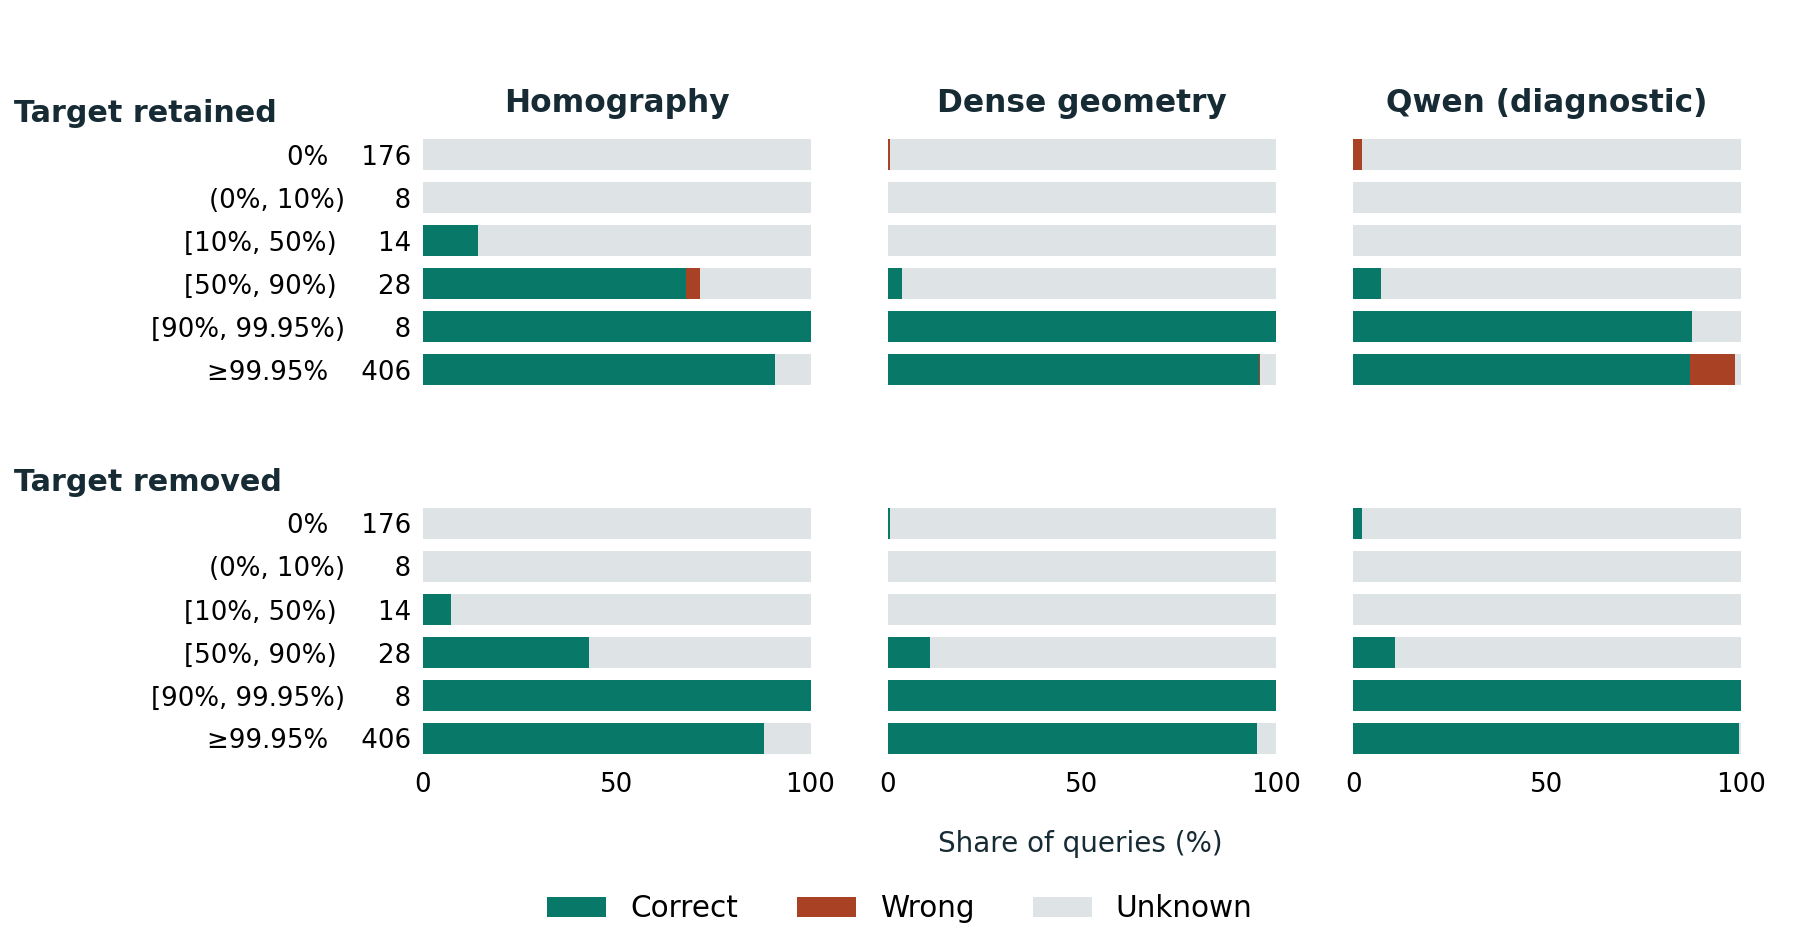
\includegraphics[width=\linewidth]{figures/answers-by-visibility.png}
  \caption{Decisions by the exposure of the retained twin, pooled across simulators. Each row gives the number of queries per physical state. Green counts correct answers, rust wrong answers and gray abstentions. At zero exposure every definite answer came from an identical MuJoCo pair. The guess was physically correct on one twin.}
  \label{fig:visibility}
\end{figure}

\subsection{Trained STILL versus zero-shot Qwen on the archived panel}
\label{sec:still}

\begin{table}[htbp]
  \centering
  \caption{Deletion decisions at the tested operating points. Each engine contributed 320 removed and 320 retained targets. Withholding deletion on a removed object counts as a miss. The final column counts identical MuJoCo pairs on which the system deleted both states.}
  \label{tab:deletion}
  \begin{tabular}{lrrr}
    \toprule
    System & \shortstack[r]{Misses\\ / 640 removed} &
      \shortstack[r]{False deletions\\ / 640 retained} &
      \shortstack[r]{Deleted both\\ / 88 pairs} \\
    \midrule
    \DeletionRows
    \bottomrule
  \end{tabular}
\end{table}

STILL detected 462 of 640 removals and zero-shot Qwen detected 419 (Table~\ref{tab:deletion}).
The difference in missed-removal rates, STILL minus Qwen, was $-6.7$ percentage points (paired 95\% layout interval, $-11.6$ to $-2.2$). The corresponding false-deletion difference was $-2.3$ points ($-8.6$ to $+4.2$). These intervals hold the development threshold fixed. The 16 layouts give clearer evidence of a difference in misses than in false deletions.

The original Qwen alignment check admitted 419 removed and 415 retained queries. Qwen found all 419 removals and erased 51 retained targets. On the same 834 queries, STILL found 405 and erased one. Among the 446 queries Qwen's gate rejected, STILL detected another 57 removals and erased 35 retained targets. Missing crops accounted for 153 of STILL's 178 misses.

The retained-target masks show where the systems failed. Qwen falsely deleted 47 fully exposed and four fully hidden targets. STILL falsely deleted 28 fully hidden and eight partly visible targets.
On the 88 identical pairs, Pi3 supplied usable crops for 16. STILL deleted both states on 11 pairs, scored below threshold on five, and withheld deletion for lack of a crop on 72. The more conservative crop threshold deleted both on one pair (Figure~\ref{fig:still-crops}). Adding the whole-scene score raised that count to 79. On this balanced set, each such deletion decision erases one valid memory.

\begin{figure}[htbp]
  \centering
  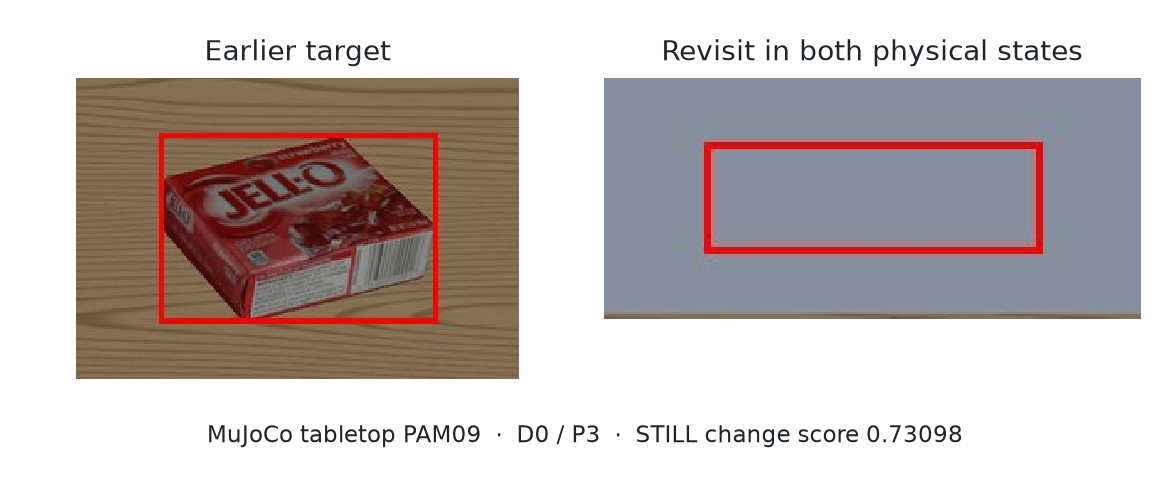
\includegraphics[width=.80\linewidth]{figures/still-registered-pair.png}
  \caption{The crops supplied to trained STILL at MuJoCo tabletop PAM09, nominal stop P3. The registered place shows the panel whether the gelatin box remains or has been removed. STILL assigned both states a change score of 0.73098. This was the only identical pair above the conservative threshold. Both geometric methods abstained.}
  \label{fig:still-crops}
\end{figure}

\paragraph{A clear-view control for interpreting Qwen.}
On 80 retained MuJoCo queries the unmarked reference and revisit were identical within the query. Both geometric verifiers found the object on all 80. Qwen deleted it on seven. Smaller visible targets accounted for most of its false deletions (Appendix~\ref{app:geometry}). We also tested a simple binary decision after inspecting the outcomes. On the 834 queries admitted by registration, a dense match score below 0.60 found the same 419 removals as Qwen and erased six retained objects. This diagnostic shows why Qwen's aggregate errors alone give weak evidence about occlusion.

\section{Discussion}

Improved alignment helped when camera motion made a clear removal difficult to recognize. The same registration could succeed on a panel that covered the remembered place. An appearance mismatch at that location then led the verifier to erase a retained object. The parked-blocker error also shows why an audit focused on occlusion needs ordinary clear controls.
STILL found 63 more removals than dense geometry but falsely deleted 34 more retained targets. Which operating point is preferable depends on the cost of leaving a stale record and the cost of erasing a valid one.

Another view can supply different evidence. In a post hoc replay of 640 blocker-placed starts, homography made 196 correct updates with one view. Choosing the most exposed alternative using an evaluator mask raised this to 292, with one false deletion under either rule. The ceiling was 319. This replay reused the inspected layouts and ignored travel costs. The proposed study on fresh layouts ended at design (Appendix~\ref{app:replay}).

Camera and room changes affected which views reached Qwen. On eight fresh service-corridor layouts, the declared oblique view yielded zero double-removal calls on eight identical MuJoCo pairs. A secondary frontal view yielded seven. When the same layouts became a furnished workshop, registration rejected all eight frontal pairs. The room changes altered several cues together (Appendix~\ref{app:rooms}).

\section{Limitations}
\label{sec:limitations}

The main audit covered two target meshes, two blocker families and one lighting condition per engine. Both engines used the same layouts and camera trajectories. The 16 independent layout units limit precision, especially for individual environments and objects. The corridor and furnished workshop reused eight layouts while changing several visual cues at once. These comparisons cannot attribute a failure to a single room feature or to model training alone.

Removing render geometry gives a controlled static intervention. It omits contact, settling, relocation and deformable occluders. The study supplies no real-camera risk estimate. Object-level changes in more varied scenes and physical captures would extend that scope.
Exact equality certifies ambiguity for one subset. Different pixels may reflect a visible target, shadows, sampling or other renderer effects. Our fixed-camera photometric calibration detected all 20 clear interventions per simulator but missed its required yield on partly occluded views. In one shelf layout a three-pixel-wide sliver supplied too little local evidence to pass the calibration (Appendix~\ref{app:calibration}). Independent visual-support judgments and additional same-state repeats would be needed to interpret the unequal pairs.
Within the tested interface, the exact pairs identify where a deletion must erase a retained object in one physically possible scene.

\clearpage
\acknowledgments{Codex and Terra assisted with implementation, simulator operation, computational review and manuscript preparation. Claude reviewed the claims and performed the retrospective extra-view analysis. AI assistants checked both analysis implementations within the same project. Simulator interventions supplied physical-state labels. Pixel comparisons tested exact equality.}
\bibliography{references}

\clearpage
\appendix
\section{Scene construction and exploratory qualification}
\label{app:design}

The shelf and tabletop use the same target meshes, object transforms and cameras in both simulators. Each layout has a block of 32 reserved development seeds. The generator takes the first seed that meets its geometric, framing and duplicate checks. Feasibility trials used separate seeds. A pudding box failed to fit the shelf before collection. The final gelatin box and marker were new target identities relative to the exploratory comparison.

Each of five nominal stops supplies a clear retained reference. The direction of the horizontal translation and the sign of yaw cycle across layouts and stops. In Isaac Sim 6.2.0.0, USD visibility controls whether RTX renders the target. In MuJoCo 3.17.0, the target geoms move to an excluded rendering group. Mesa llvmpipe renders the scene. Both interventions retain the object definition and nominal transform. An enabled flag records the intervention, and native instance masks record visible target pixels. A fully hidden retained object can have an empty visible mask.

Each renderer produces $2304\times1296$ RGB. Lanczos resampling delivers $1200\times675$ inputs. The numeric reference box encloses the scaled, half-open native bounds. The inference call excludes filenames, pairing information, interventions, masks, camera parameters and registration ground truth. Each original verifier independently scored each member of a pair. The evaluator compared both complete decoded images and the box across states and repeated the image check at native resolution.

\begin{figure}[htbp]
  \centering
  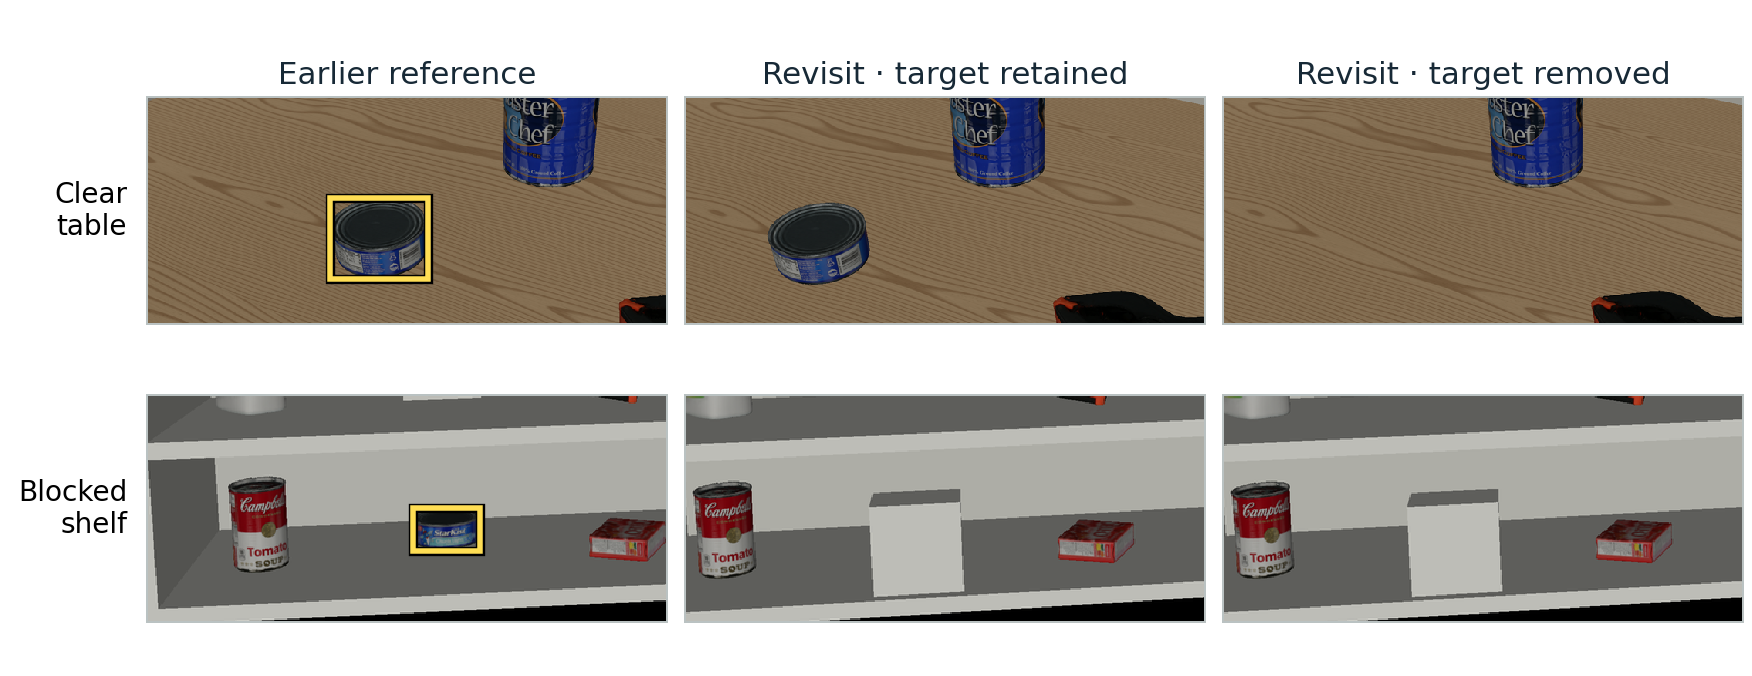
\includegraphics[width=\linewidth]{figures/counterfactual-example.png}
  \caption{Exploratory MuJoCo examples. The outline marks the remembered tuna can. Changing its state alters 12,159 of 810,000 pixels in the tabletop revisit. On the shelf all 810,000 revisit pixels match. The verifier sees one revisit per query. These crops illustrate the intervention.}
  \label{fig:exploratory}
\end{figure}

The exploratory set comprised ten layouts, five per environment, with three camera-motion magnitudes and five stops. At the largest motion, dense geometry found 25/25 clear tabletop removals in each simulator. Homography found 17/25 in Isaac Sim and 16/25 in MuJoCo. Across 1,200 queries, dense geometry gained 113 correct answers and lost 70 relative to homography. It introduced two false deletions of the same retained foam brick at one MuJoCo shelf stop, with the blocker parked and placed. On another fully blocked shelf pair, homography reported removal in both worlds (Figure~\ref{fig:exploratory}). These observations informed the choice of main endpoint and controls.

\section{Verifier settings and capability screens}
\label{app:operating}

\paragraph{Geometry.}
The homography uses a coarse-to-fine enhanced correlation coefficient fit to image edges outside the target neighborhood~\citep{ecc}. Dense geometry estimates camera pose and depth and discards out-of-frame, invalid and depth-inconsistent projections~\citep{vggt,geoscd}. After registration, both methods compare DINOv2 patch features and estimate obstruction from detections and local foreground and background changes~\citep{dinov2,yoloworld}. Registration must pass and local quality must reach 0.30. A similarity of at least 0.70 gives \emph{present}. A similarity of at most 0.60 with obstruction at most 0.40 gives \emph{removed}. All other cases give \emph{unknown}.

\paragraph{Zero-shot Qwen.}
The reader receives two $768\times432$ scene images with the reference box marked, a reference crop, and a warped revisit crop. Each crop fits within $512\times512$ pixels. Although the prompt describes the reference crop as enlarged, preprocessing only downsizes oversized crops. Black pixels in the warped crop denote locations without a mapping. The reader uses greedy decoding and a parser for three literal answers.
The development screen required at least 34/36 correct identical-view answers and 36/40 correct per clear class. Qwen scored 36/36 on unchanged references, 40/40 on clear retained targets, and 40/40 on clear removals. Each simulator supplied 20 of each clear class across nominal and moved cameras. All outputs parsed. The median reference box area was 9,496.5 pixels in the screen and 6,666 on main inputs admitted by registration. The screen contained no hidden targets.

\paragraph{Trained STILL.}
The authors' seed-2 verifier scores the first-token probability of change in red-box crops~\citep{still,still-weights}. Pi3 estimates a projected box from the two RGB images~\citep{pi3}. A crop must have nondegenerate bounds and pass the authors' 0.30 visibility cutoff. We use a constant proposal weight because the target and reference box are supplied. The original SD-V detector also uses proposal confidence. We scored each distinct input tuple once within a split and restored every case to its original position for evaluation.

Development supplied 400 retained and 400 removed queries. Selecting the place threshold for maximum removal F1 gave 0.00071. Selecting it for zero development false deletions gave the conservative value of 0.11916. A third rule uses the geometric mean of the scene and place change scores when a crop exists, and the scene score alone otherwise. Its development-selected threshold was approximately 0.0003872983. The original authors used a threshold calibrated on their own detection scenes. Our binary endpoint counts a withheld deletion on a removed target as a miss. It counts a deletion of a retained target as a false deletion.

\section{Geometric and zero-shot outcomes by simulator}
\label{app:geometry}

\begin{table}[htbp]
  \centering
  \caption{Original three-output verifiers on every main intervention. Each simulator supplied 640 queries, including 320 retained and 320 removed objects. Correct and definite counts include both states. A false presence asserts that a removed object remains.}
  \label{tab:coverage}
  \begin{tabular}{llrrrr}
    \toprule
    Simulator & Verifier & Correct & Definite & \shortstack[r]{False\\ removal} & \shortstack[r]{False\\ presence}\\
    \midrule
    \CoverageRows
    \bottomrule
  \end{tabular}
\end{table}

On clear moved-camera shelf removals, both geometric methods scored 37/40 in Isaac Sim. The score rose from 33/40 to 38/40 in MuJoCo (Figure~\ref{fig:targets}). Across all interventions, dense geometry gained 26 correct answers and lost 16 in Isaac Sim. It gained 38 and lost 27 in MuJoCo. The three original verifiers completed all 3,840 evaluations. An always-abstaining rule gives zero correct answers and zero errors. Always reporting removal gives 80/80 on the clear moved-camera removal endpoint and falsely deletes all 320 retained objects per simulator.

\begin{figure}[htbp]
  \centering
  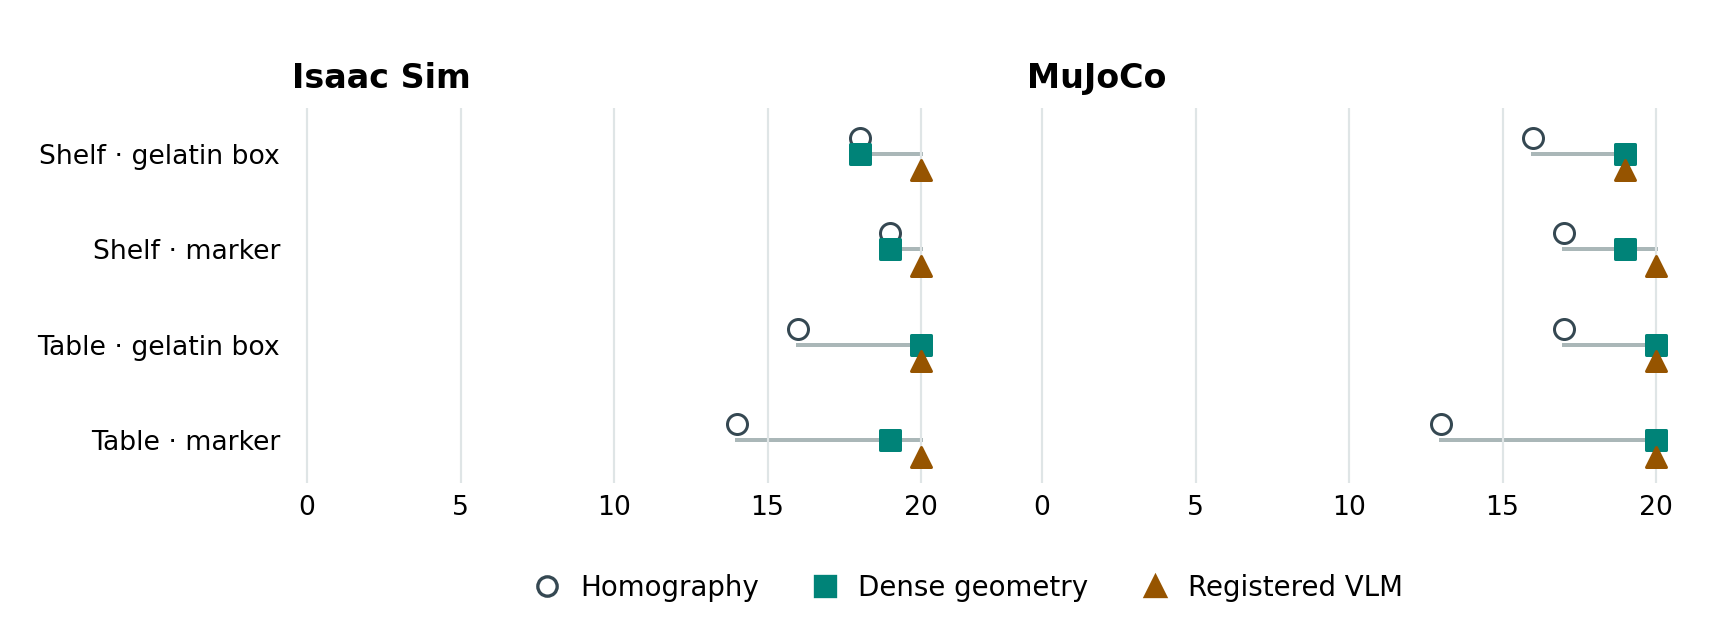
\includegraphics[width=.94\linewidth]{figures/primary-by-target.png}
  \caption{Correct clear removal decisions after camera motion. Each group contains four layouts and five stops per layout. Offset markers show equal counts.}
  \label{fig:targets}
\end{figure}

\begin{table}[htbp]
  \centering
  \caption{Identical retained/removed input pairs by simulator. The last three columns count definite decisions on both twins by the original systems. A dash denotes an empty comparison set.}
  \label{tab:exact}
  \begin{tabular}{lrrrrr}
    \toprule
    Simulator & \shortstack[r]{Identical\\ / all pairs} & \shortstack[r]{Layouts\\ with a pair} & Homography & \shortstack[r]{Dense\\ geometry} & \shortstack[r]{Zero-shot\\ Qwen}\\
    \midrule
    \ExactRows
    \bottomrule
  \end{tabular}
\end{table}

The wide panel completely hid the target at 76/80 placed positions per simulator, and the white box did so at 12/80. None of the 160 parked-blocker pairs per simulator produced identical inputs (Table~\ref{tab:exact}). At MuJoCo shelf PAM05, stop P5, local image quality was 0.737 on the identical pair that dense geometry deleted. Qwen's gate admitted four exact pairs across PAM01, PAM02 and PAM05. All four used the wide blocker, the moved camera, and stop P4 or P5. The gate stopped both members of every other exact pair.

Across all 640 pairs, 176 were completely hidden. Another 402 had full exposure, and four had at least 99.95\% but less than full exposure. The remaining 58 pairs fell between those groups. Of the 51 Qwen false deletions, 29 came from the nominal camera pose. Among the 406 retained targets with at least 99.95\% exposure, Qwen's false deletions by increasing thirds of native silhouette area were 33/135, 10/135 and 4/136. Target identity, layout and size varied together.

Zero-shot Qwen found 80/80 clear moved-camera removals in Isaac Sim and 79/80 in MuJoCo. It also falsely deleted 11 parked-blocker retained targets per simulator. In every parked-blocker retained query, at least 99.96\% of the native silhouette was exposed. Among the 834 queries admitted by the shared gate, Qwen itself abstained twice. Dense geometry found 399/419 removals and erased 2/415 retained objects. It correctly reported \emph{present} on 42 of Qwen's 49 additional false deletions.

\section{What the fixed-camera calibration measures}
\label{app:calibration}

Four separate layouts used a tuna can or foam brick and a side-offset blocker. A base render, two fresh repeats and a distractor-only change accompanied each intervention. The evaluator selected a $7\times7$ patch inside the intersection of the reference mask and the exposed retained-target mask. At least 25 pixels had to qualify. Their mean absolute RGB change had to reach 8 on the 0--255 scale and exceed the larger first-repeat difference by at least 4. Second repeats and distractor changes in each physical state served as negative controls. The screen required zero false triggers, at least eight of ten clear pairs per environment and engine, and a partly visible positive pair in every layout.

The check detected all 20 parked-blocker target interventions per simulator. Each also supplied 13 eligible placed pairs and 132 eligible negative controls. None of these controls triggered. For the remaining 28 of 160 planned negative comparisons per simulator, the evaluator found no eligible patch. Whole-image change exceeded both repeats on 74/80 Isaac Sim and 72/80 MuJoCo distractor manipulations.

Both simulators missed the required yield on partly visible targets. The shelf can in PAC01 produced three fully exposed views, one fully hidden view and one sliver. In MuJoCo, the sliver occupied three native columns and 74 of 6,155 isolated target pixels. No $7\times7$ patch could contain 25 target pixels (Figure~\ref{fig:sliver}). Successful partly visible sites in the other three layouts exposed approximately 48.4\%, 1.9\% and 97.8\% of the silhouette. Only the first falls between 10\% and 90\%.

\begin{figure}[htbp]
  \centering
  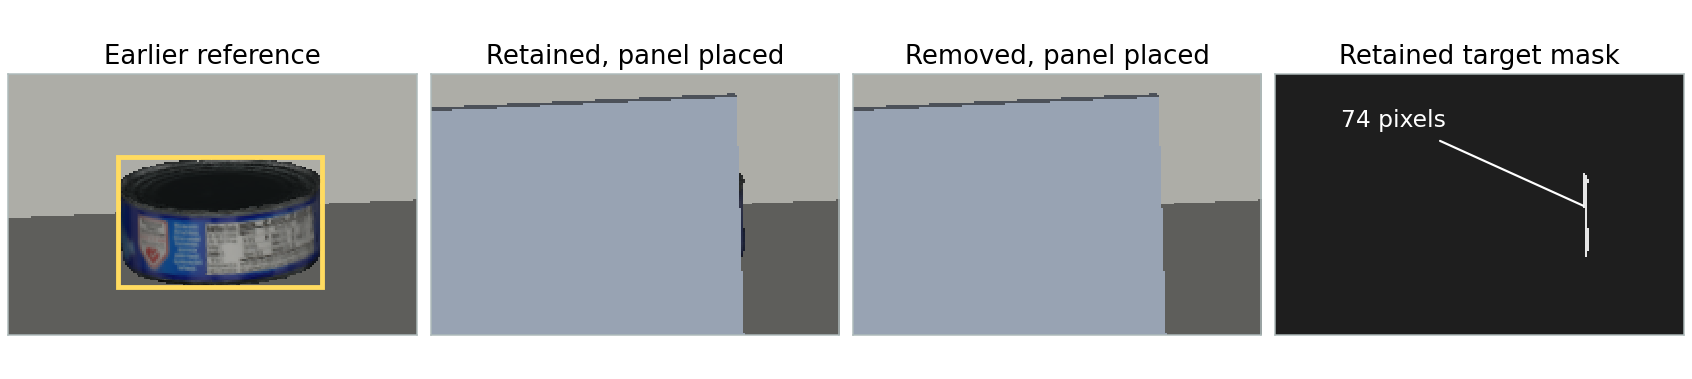
\includegraphics[width=\linewidth]{figures/calibration-sliver.png}
  \caption{Fixed-camera MuJoCo calibration. Only a sliver of the retained can is visible beyond the panel. The right-hand view shows native instance-mask pixels available to the evaluator.}
  \label{fig:sliver}
\end{figure}

Changing the midpoint convention for a half-open box changed seven local contrast values across the two engines. All positive-pair and qualification verdicts stayed the same. Five calibration pairs per simulator had zero visible target pixels. In Isaac Sim the median whole-image mean absolute difference at scoring resolution was 0.321 intensity levels across physical states and 0.326 within same-state repeats. Both medians were zero in MuJoCo.

\paragraph{Why the hidden Isaac Sim images differ.}
We reexamined the 88 fully hidden pairs from the main panel at native resolution. Across the recorded object, shelf and camera fields, only target visibility differed between twins. The blocker mask covered the entire isolated target silhouette at every position. A pixel counted as changed if any RGB channel differed. The median share of changed pixels was 59.2\%, yet the median whole-image mean absolute difference was only 0.293 intensity levels. On 80 unchanged nominal views with the blocker parked, the corresponding median was 0.309. A median of 99.66\% of changed pixels fell outside the target's isolated silhouette, which itself occupies only a small part of the frame.

To check for reproducible local changes, we revisited the five fully hidden calibration views in a post hoc analysis. We divided each original image pair into disjoint $16\times16$ native-pixel tiles and selected the tile with the greatest absolute difference in mean intensity across states. We then evaluated the same tile in two additional archived render pairs at that camera. In four views the tile was brighter after removal on both repeats and lay entirely outside the target and blocker footprints. Its smallest contrast across states exceeded its largest range within either state. The fifth tile reversed sign on one repeat. Figure~\ref{fig:indirect} shows the largest base contrast. A change in indirect lighting is plausible. Capture always rendered the placed, retained state before the placed, removed state, and there was no lighting ablation. These captures cannot identify a specific rendering mechanism or assign a cause to each of the 88 main pairs.

\begin{figure}[htbp]
  \centering
  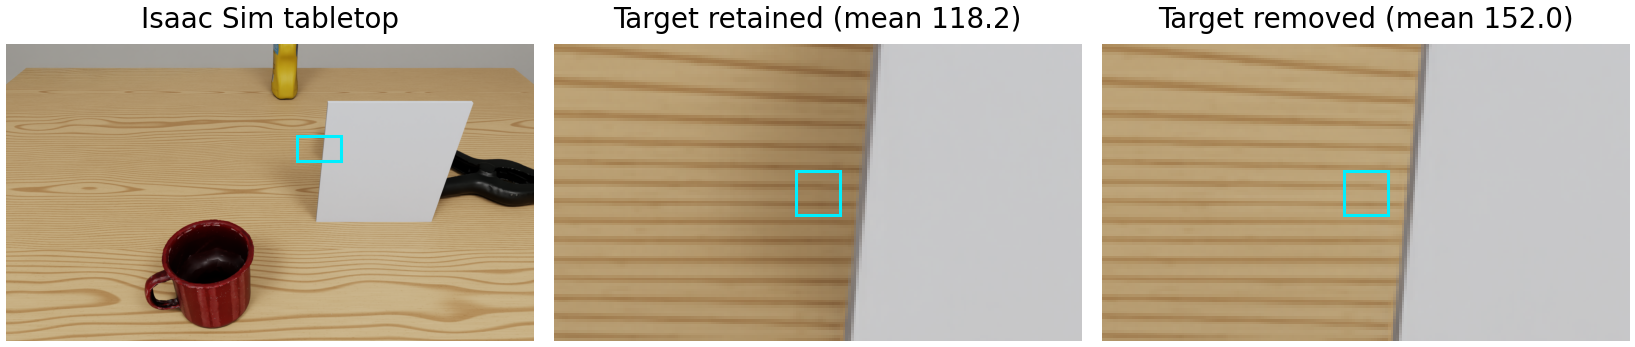
\includegraphics[width=\linewidth]{figures/isaac-hidden-patch.png}
  \caption{Isaac Sim calibration, tabletop PAC04, stop P3. The left outline locates the enlarged crops. The crop outlines mark the same $16\times16$ tile on the exposed tabletop. The tile was 33.9 levels brighter in the removed frame of the base pair and 34.3 and 33.4 levels brighter in the two repeats. The retained foam brick was entirely hidden.}
  \label{fig:indirect}
\end{figure}

\section{Camera and room sensitivity}
\label{app:rooms}

Four previously identified MuJoCo shelf pairs again elicited removal on both states from the zero-shot system at their original camera angles. Rotating each camera in place to level the shelf edge caused registration to reject all four pairs. The language model then received none of them.

Eight fresh service-corridor layouts placed a bottle or drill behind a sliding door. The declared oblique test produced zero double-removal calls on eight identical MuJoCo pairs. A secondary frontal view gave seven on eight pairs. Both camera position and heading changed.

The furnished workshop revisited the same eight layouts after changing the room and door bay. Its declared frontal test gave zero double-removal calls on eight identical MuJoCo pairs. All eight failed registration. Homography classified all 80 open-door controls correctly in each simulator and abstained on every closed-door query. The zero-shot system found all 40 open-door removals per simulator. It falsely deleted an exposed drill on 4/40 retained queries in Isaac Sim and 2/40 in MuJoCo. All six errors occurred on the two added robot camera mounts. The corridor and workshop share layouts, and the furnishing, light and door geometry changed together.

\section{Retrospective replay with a reference at each stop}
\label{app:replay}

The archived panel contains five stops for each combination of simulator, layout, camera-motion level, blocker position and target state. The replay kept any definite homography answer across 640 blocker-placed starts. After an abstention, it took the saved answer from one of the other four stops while holding the other conditions fixed. That answer used the alternate stop's own earlier reference image, target box, and revisit. Across the 1,772 alternate-stop choices for the 443 homography abstentions, both the reference image and its box differed from those at the starting stop.

The starting stop alone gave 196/640 correct decisions (30.6\%). A uniform choice among the alternatives averaged 268.5 (42.0\%). Choosing the alternative with the greatest exposure in the retained twin's evaluator mask gave 292 (45.6\%). The starting and mask-assisted rules each made one false deletion. A ceiling that used both the true state and every alternative's answer reached 319 (49.8\%). These numbers describe a system that stores a reference at each stop and switches to a second reference/revisit pair after abstaining. Evaluating an extra revisit with a single stored reference would require scoring the new revisit against the starting reference and box. The replay used the inspected layouts and omitted travel costs. The proposed study on fresh layouts ended before collection.

\section{Relation to other evaluation designs}
\label{app:related}

PBD-AG tests false absence in robot memory by requiring repeated observable misses based on measured depth~\citep{pbdag}. A robot using SafeVantage can seek evidence from reachable viewpoints under a travel budget~\citep{safevantage}. VA-TAMP obtains observations for actions that depend on uncertain object models~\citep{vatamp}. Our interface fixes a previously identified object, its earlier RGB box and one revisit. With these inputs, certainty about a particular deletion can be tested without choosing a new action.

TRAPSBench pairs answerable and unanswerable physics questions. The Counterfactual Memory Audit varies the available history while fixing the current observation~\citep{trapsbench,cma}. Our intervention holds the supplied history fixed too. SpatialUncertain uses geometry and human screening to evaluate reasoning on occluded views and includes a separate task on perspective and apparent size~\citep{spatialuncertain}. VAD-R studies when models refrain from answering without being prompted to abstain~\citep{vad-r}. Our zero-shot system receives an explicit unknown option. These tasks motivate separating an accurate guess, a supported update and an abstention.

\section{Data and reproducibility}
\label{app:data}

The \href{https://github.com/Adithya-Rajendran/cmpe249-active-verification/releases/tag/scene-memory-audit-v1}{versioned data release} contains the delivered RGB images and their hashes, native renders with evaluator masks, target assignments, case and pair tables, primary protocol, calibration measurements and original scorer outputs. It includes a second analysis implementation from the same project. The visibility analysis and alternate-stop replay reuse these archived cases.

The \href{https://github.com/Adithya-Rajendran/cmpe249-active-verification/blob/a88d89fc5c92f4f18f7a7a1d5947bc59f3b37161/paper/README.md\#reproduce-the-trained-still-comparison}{trained-comparison guide} provides the development and main probabilities, registered boxes, operating points, restored per-query decisions, inference commands and CPU recount. It identifies the exact \href{https://huggingface.co/oran9er/STILL-Qwen3.5-9B/tree/81d9373e1dd9c07c537d5fb2436b36a26a2206b4}{trained STILL} and \href{https://huggingface.co/Qwen/Qwen3.5-9B/tree/c202236235762e1c871ad0ccb60c8ee5ba337b9a}{zero-shot Qwen} model revisions~\citep{still-weights,qwen-weights}. The labels record the simulator intervention. No human annotated support on unequal inputs.

\end{document}
